\section{Introduction}
\label{sec:intro}

\subsection{Association}
The association Akademische Raumfahrt Initiative Schweiz (ARIS) brings together students from Swiss universities fascinated by space exploration. Formed around ETH Zurich, HSLU, ZHAW, UZH and OST the association engages it's members in engineering challenges by integrating theory and practice. ARIS is also offering a wide variety of Theses for parts and systems that can be integrated in their future rockets. 

\subsection{Background}
In order to reduce the drift of a sounding rocket's descent a multi stage recovery system is needed. Normally, at apogee, a drogue chute is deployed, and the main chute is released at a lower altitude. If a parachute inflates too rapidly it can cause extreme shock to the overall parachute system and rigging causing it to malfunction. In order to keep the loads to a minimum, the descent speed needs to be reduced but at the same time the rocket needs to come down to earth as fast as possible to reduce its drift. As the rockets developed by ARIS get bigger and heavier new methods need to be developed to reduce these loads.\newline
Reefing is something that prevents a parachute from opening too rapidly. With an active reefing system the main parachute can be deployed at apogee and slowly open at a low altitude. This would simplify and reduce the overall weight of the recovery system.
\medskip
\begin{figure}[h!]
	\centering
	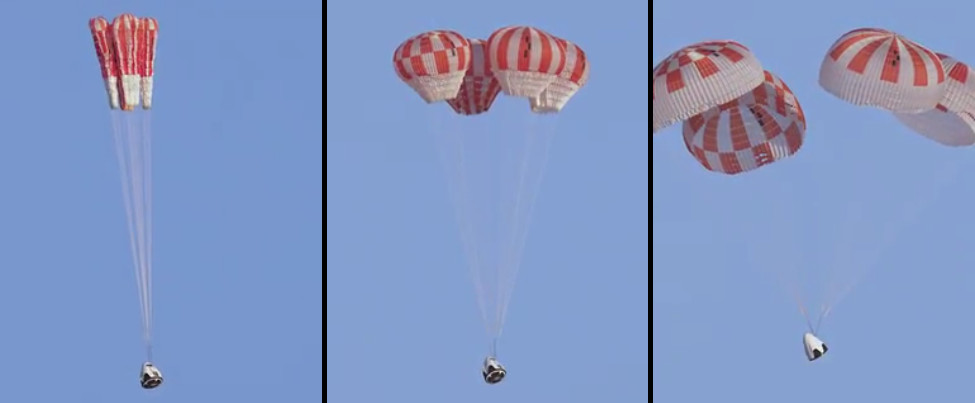
\includegraphics[height=6cm]{images/dragon.jpg}
	\caption{Dragon Reefing System}
	%\vspace{-2ex}
	%\caption*{\textbf{Source:} Original task definition}
	\label{fig:dragon_parachute}
\end{figure}

In the space industry reefing is often achieved by cutting lines inside the parachute. In the \cref{fig:dragon_parachute} above two lines are cut inside the parachute. This is often done by using pyrotechnic line cutters, activated by an electric signal.